%% ---------------------------------------------------------------------------
%%  Context-Dependent Selection of Urban Routing Policies
%%  IC_TORS'26 submission manuscript.  Standalone: compile main.tex directly.
%%    pdflatex main -> bibtex main -> pdflatex main -> pdflatex main
%%  Figures are external PDFs in figures/.  Tables are inline.
%% ---------------------------------------------------------------------------
\documentclass[runningheads]{llncs}

\usepackage[T1]{fontenc}
\usepackage[utf8]{inputenc}
\usepackage{lmodern}
\usepackage{amsmath,amssymb}
\usepackage{graphicx}
\usepackage{booktabs}
\usepackage{tabularx}
\usepackage{array}
\usepackage{microtype}
\usepackage[hidelinks]{hyperref}
\usepackage{url}

\renewcommand{\UrlFont}{\ttfamily\small}
\newcommand{\CO}{CO\textsubscript{2}}
\newcolumntype{R}{>{\raggedright\arraybackslash}X}
\setlength{\tabcolsep}{4pt}

\begin{document}

\title{Context-Dependent Selection of Urban Routing Policies:\\
Regime Effects, Decision Value and Generalisation Limits}
\titlerunning{Context-Dependent Selection of Urban Routing Policies}

\author{Anonymous author(s)}
\authorrunning{Anonymous submission}
\institute{Affiliations withheld for review}

\maketitle

\begin{abstract}
Route guidance systems normally commit to one routing objective before any trip is
planned, even though the relative merit of established objectives can depend on the
traffic state. This paper studies the selection of the routing \emph{policy} rather than
of a route. Using 432 completed SUMO simulations over 24 controlled contexts on a
twelve-signal urban mesh, we evaluate shortest-distance routing (SP), dynamic
travel-time routing (DTT) and constrained travel-time-aware eco-routing under three
demand levels, four restriction configurations and two signal plans, with preference
expressed as a fixed-reference additive cost over mean journey time and tailpipe \CO.
SP has the lowest observed cost in all eight low-demand contexts and DTT in all eight
high-demand contexts, and the signal plan displaces the crossing by at least one step of
the demand grid. Relative to the single best fixed policy, leave-one-context-out
selection lowers mean decision regret from 0.03018 to 0.00606 normalised cost units ---
79.9\,\% of the available decision headroom captured, with the lowest-cost policy chosen
in 21 of 24 contexts. A two-threshold rule on demand and signal plan reproduces that
result exactly, so the benefit follows from the regime structure rather than from model
capacity. A leave-one-demand-out test reverses the conclusion: pooled regret rises to
0.07649, above the fixed-policy benchmark. Policy selection therefore has measurable
value inside the regimes represented during fitting and can be worse than a fixed policy
outside them. The contribution is the empirical characterisation of this decision
boundary and its limits; no new routing, multi-criteria or learning algorithm is
proposed.
\keywords{Routing-policy selection \and Urban traffic simulation \and Algorithm
selection \and Decision regret \and Traffic regimes \and Generalisation.}
\end{abstract}

\section{Introduction}

A route guidance system makes two decisions that are easy to conflate. The first is
the classical route-choice problem: which path should a vehicle take from an origin to
a destination? The second is rarely treated as a decision in its own right: which
routing \emph{policy} should generate that path? An operator may minimise static
distance, respond to recently observed travel times, or minimise estimated emissions
subject to a travel-time budget. Each policy returns a different path for the same
request, so the choice of policy precedes and constrains the choice of route. This
paper studies the second decision.

The distinction matters because congestion changes the relative value of routing
objectives. On a lightly loaded network the shortest path is usually also fast, and
minimising distance gives up little. As load rises, repeated concentration of traffic
on the shortest corridor raises delay there faster than on the alternatives, and a
policy that reacts to observed travel times can become preferable. Signal timing
modifies the same relationship, because the green split determines how much capacity
each competing movement receives. These mechanisms are individually well documented at
the level of routes and traffic dynamics, but they do not answer the question an
operator faces: should one routing objective be fixed for the whole day, or should the
active objective change with the operating context, and how much is that change worth?

We treat this as a context-dependent algorithm-selection problem in the sense of
Rice~\cite{rice1976algorithm}. The object being selected is a routing policy, not a
route: each policy remains responsible for assigning paths according to its own
objective, and a context-aware layer only decides which policy is active for the
current operating episode. Separating the two levels makes it possible to measure the
value of adapting the policy without attributing it to any particular route-generation
mechanism.

The central research question is:

\begin{quote}
\emph{Under which traffic regimes does the preferred established routing policy
change, how much decision value is available from adapting that policy, and how
reliably can the resulting structure be identified on unseen contexts?}
\end{quote}

Three subsidiary questions follow. How does the signal plan move the demand range in
which the preferred policy changes? How much of the available decision headroom can a
simple interpretable rule recover on held-out contexts, and does a flexible model
recover more? And what happens when the rule is applied outside the range of operating
conditions represented while it was fitted?

The paper makes four empirical contributions on a benchmark of 432 completed
simulations. It characterises a regime-dependent preference structure among established
routing policies on a signalised network, and shows that the signal plan displaces the
switching range by at least one step of the tested demand grid. It quantifies the value
of adaptation with context-level decision regret against a hindsight benchmark rather
than with prediction error, and reports how that value is distributed across regimes. It
shows that a two-threshold rule on demand and signal plan attains the same held-out
decision quality as a fitted regression tree, which bounds what the learned model
contributes. And it identifies an explicit generalisation boundary: the procedure that
helps inside the represented regime space becomes worse than the fixed policy it
replaces when an entire demand regime lies outside it. No new routing algorithm,
multi-criteria method or learning method is proposed, and no claim of priority is
made.

\section{Literature Review}

The relevant work spans three strands. Each is summarised below in terms of what it
establishes; the third closes with the position of the present study.

\subsection{Dynamic and Traffic-Aware Routing}

Shortest-path computation on a static network is the classical starting
point~\cite{dijkstra1959note}. Dynamic routing replaces static link attributes with
time-dependent or observed travel times, and stochastic formulations treat network
conditions as random and solve for routing policies rather than fixed
paths~\cite{gao2006optimal,levering2021framework}. Proactive rerouting distributes
vehicles over alternatives to relieve anticipated congestion, and stochastic
optimal-control formulations extend this to uncertain demand and heterogeneous
behaviour~\cite{pan2013proactive,pi2017stochastic}.

A second body of work establishes that the benefit of traffic information depends on the
operating state. Empirical studies of real-time rerouting report larger gains during
congested periods and for trips whose alternatives materially change experienced travel
time~\cite{falek2021reroute}; simulation and analytical studies identify demand-dependent
transitions in the effectiveness of dynamic guidance, including regimes in which
rerouting ceases to help~\cite{novikov2018dynamic,routing2026phase,chen2025detour}; and
work on route choice under different control systems shows that the control regime itself
can change the relative performance of route-choice
strategies~\cite{xie2014unified,papageorgiou2003review}. What this literature does not
establish, and what is measured here, is where the \emph{preference order} between
established policies reverses as a joint function of demand and signal plan, and what an
operator gains by acting on that reversal rather than by improving any single mechanism.

\subsection{Environmental, Multi-Criteria, and Context-Dependent Routing}

Environmental routing incorporates emissions or fuel use into path costs using historical
or real-time traffic information~\cite{boriboonsomsin2012ecorouting,zeng2016prediction}.
Because a minimum-emission path can be much slower than the fastest path, emission
objectives are commonly constrained by a travel-time budget, producing the constrained
eco-routing family used here~\cite{zeng2017svm,huang2018ecorouting}; vehicle-specific
formulations show further that the relationship between route choice, traffic state and
emissions depends on vehicle and network characteristics~\cite{wang2019ecorouting}.

The multi-criteria literature supplies established ways of representing preferences over
competing outcomes, including additive value models and outranking or compromise
methods~\cite{keeney1993decisions,hwang1981multiple,opricovic2004compromise,%
brans1985preference,ehrgott2005multicriteria}. Here such a model is used only to make
``preferred policy'' operational, not as a contribution, and the check it implies ---
reported in Section~\ref{sec:robust} --- is whether the chosen criteria discriminate among
the candidate policies at all, since a preference model that changes no decision adds
nothing however sophisticated. What is measured here is whether the two primary criteria
are sufficiently independent in a signalised urban setting for a preference model to
matter, and whether a third, system-level congestion criterion changes which policies are
mutually incomparable.

\subsection{Algorithm Selection and Decision-Oriented Evaluation}

The algorithm-selection framework formalises the observation that different algorithms are
preferable on different problem instances, and that instance features can be mapped to
expected performance~\cite{rice1976algorithm}; portfolio systems operationalise this and
benchmark libraries standardise how they are
evaluated~\cite{xu2008satzilla,bischl2016aslib,kotthoff2014survey}, while instance-space
analysis shows how performance varies across the problem space~\cite{smithmiles2023isa}.
Two reference points from that literature are used throughout: the single best fixed
algorithm, the strongest deployable non-adaptive choice, and the virtual or hindsight
best, which selects per instance using knowledge available only after the fact. A second
relevant distinction is between predictive accuracy and decision quality: a model may
predict poorly yet decide well when the ranking of alternatives is preserved, while a small
prediction error can be costly if it changes the selected
alternative~\cite{elmachtoub2022smart}. This motivates evaluating a selector by decision
regret against the per-instance best~\cite{kouvelis1997robust} rather than by regression
error.

\paragraph{Position of this study.}
The three strands meet at a question none answers alone. The routing literature
establishes that policy performance is state-dependent but compares mechanisms rather than
deciding among them; the multi-criteria literature supplies preference models but does not
test whether they discriminate in a given environment; the algorithm-selection literature
supplies the decision-theoretic apparatus but has not been applied to routing policies
under controlled traffic regimes. This study occupies that intersection and contributes no
new mechanism --- the policies are established objectives, the preference model is a
standard fixed-reference additive cost and the selector is a shallow regression tree. What
is new is the measurement: a controlled, fully replicated characterisation of when the
preferred routing policy changes, what that change is worth in decision terms, how little
model capacity is needed to exploit it, and where the resulting rule stops being valid.

\section{Problem Formulation}

\subsection{Contexts, policies and the two-level decision}

Let $\mathcal{S}$ be a set of operating contexts and $\mathcal{A}$ a finite set of
retained routing policies. A context $s\in\mathcal{S}$ contains only quantities known
\emph{before} the policy is activated; here it is the triple (scheduled primary demand,
planned restriction configuration, signal-control plan), and no realised travel time,
queue, flow or emission is part of it. A policy $a\in\mathcal{A}$ maps a route request to
one path from a finite admissible catalogue according to its own objective.

The decision has two levels: \emph{Level 1}, policy selection, maps the context $s$ to one
policy $a\in\mathcal{A}$; \emph{Level 2}, route assignment, is performed by that policy
according to its own objective. Only Level 1 is learned. The unit of analysis is the context, not the vehicle and not the
replication: a context is one instance in the algorithm-selection sense, all of its
replications move together through every evaluation protocol, and the selector never
observes the realised outcome of any candidate policy in the context it decides about.

\subsection{Decision cost, regret and headroom}

Let $y_{sak}$ be the mean outcome of criterion $k$ in context $s$ under policy $a$,
averaged over replications after run-level aggregation. With positive fixed references
$r_k$ and weights $w_k\ge0$, $\sum_k w_k=1$, the scalar decision cost is
\begin{equation}
C_{sa}=\sum_k w_k\,y_{sak}/r_k ,
\label{eq:cost}
\end{equation}
lower being preferred. The references are fixed for the whole benchmark rather than
recomputed per context, so costs are comparable across contexts and a context in which
every policy is slow is not rescaled into apparent equality; one cost unit is one
benchmark-average criterion value.

The best policy actually observed in a context is
$a_s^{*}\in\arg\min_{a\in\mathcal{A}} C_{sa}$, with cost $C_{s}^{\mathrm{VB}}$. Selecting
$a_s^{*}$ everywhere defines the \emph{hindsight} (virtual best) policy: a bound, not a
method, since it uses the realised performance of every candidate. For a selection rule
$\pi:\mathcal{S}\rightarrow\mathcal{A}$ the \emph{decision regret}
$R_s(\pi)=C_{s,\pi(s)}-C^{\mathrm{VB}}_{s}\ge0$ measures the cost of the decision, not the
error of a prediction. The strongest deployable non-adaptive rule is the \emph{single best
fixed policy} $a^{\mathrm{SB}}=\arg\min_{a}|\mathcal{S}|^{-1}\sum_{s}R_s(a)$, and the
quantity adaptation can win is the \emph{decision headroom} $\bar H$, of which a rule
recovers the fraction $G(\pi)$:
\begin{equation}
\bar H=\frac{1}{|\mathcal{S}|}\sum_{s\in\mathcal{S}}
\bigl(C_{s,a^{\mathrm{SB}}}-C^{\mathrm{VB}}_{s}\bigr),
\qquad
G(\pi)=\frac{\bar H-\overline{R(\pi)}}{\bar H} .
\label{eq:headroom}
\end{equation}
Thus $G=1$ for the hindsight bound, $G=0$ for the single best fixed policy, and $G<0$ for
a rule worse than doing nothing adaptive. Because $\bar H$ is defined on a finite context
set, $G$ is a benchmark-specific decision statistic. It is \emph{not} a percentage
reduction in travel time, emissions or any other physical quantity; the two are reported
separately throughout.

\subsection{Three properties that must not be confused}

\emph{Complementarity} asks whether different policies win in different contexts. It is a
property of the portfolio and environment alone, established by observing that $a^{*}_{s}$
is not constant over $\mathcal{S}$, and it says nothing about how much the variation is
worth. \emph{Decision value} asks how much cost the variation carries, and is $\bar H$ in
\eqref{eq:headroom}; a portfolio can be strongly complementary while $\bar H$ is
negligible, if the single best fixed policy is nearly optimal wherever it is not optimal,
so complementarity is necessary for decision value but not sufficient.
\emph{Deployability} asks whether the variation can be exploited from pre-decision
information on contexts not used for fitting, and is $G(\pi)$ under a held-out protocol
together with evidence about the range of contexts over which the rule remains valid;
positive decision value does not imply it, and a rule deployable on one region of the
context space need not be deployable outside it. All three are measured separately in
Section~\ref{sec:results}, and this study reports a different answer for each.

\section{Methodology}

\subsection{Simulation Environment and Network}

All experiments use one fixed topology: a bidirectional $3\times4$ signalised mesh with 12
signalised junctions, 47 external links and 29 legal simple primary paths
(Fig.~\ref{fig:network}). The upper, central and lower corridors have speed limits of 40,
50 and 60\,km/h and one, one and two lanes, so the three east--west corridors differ in
both free-flow speed and capacity, and three alternative eastbound locations carry a
150\,m speed-restriction segment with a speed ratio of 0.35. Signals run a common 60\,s
cycle: the balanced plan allocates approximately 26\,s each to the competing east--west
and north--south movements, the arterial-priority plan 36\,s and 16\,s, with identical
clearance intervals. Four background streams load the north--south movements that compete
with the primary corridors, and a three-lane source and sink ensure that neither end of
the corridor is the binding constraint. Lane counts are specified design inputs, not
calibrated saturation flows, which limits the external interpretation of absolute values.
Simulation uses SUMO~\cite{lopez2018sumo} with teleporting disabled, so a vehicle that
cannot be inserted waits rather than disappearing from the accounting.
Table~\ref{tab:config} lists the configuration.

\begin{figure}[tb]
\centering
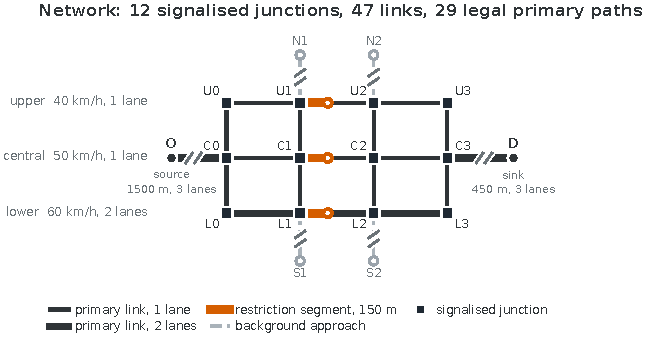
\includegraphics[width=\linewidth]{figures/fig1_network.pdf}
\caption{The fixed network. Line weight encodes lane count, the three alternative
restriction segments are highlighted, and background approaches are dashed with their
stubs shortened at the break marks. Exactly one restriction segment is active in a
restricted context. The 24 contexts built on this network are shown in
Fig.~\ref{fig:regime}b.}
\label{fig:network}
\end{figure}

\begin{table}[htb]
\centering\small
\caption{Simulation configuration. Every item is common to all 432 runs; the factors that
vary between contexts are listed in Section~5.1.}
\label{tab:config}
\begin{tabularx}{\linewidth}{@{}>{\raggedright\arraybackslash}p{0.26\linewidth}R@{}}
\toprule
Item & Setting\\
\midrule
Network & Bidirectional $3\times4$ mesh; 12 signalised junctions; 47 external links; 29
legal simple paths; 400\,m horizontal and 300\,m vertical spacing\\
Corridors & Upper 40\,km/h, 1 lane; central 50\,km/h, 1 lane; lower 60\,km/h, 2 lanes\\
Signal cycle & 60\,s, with two 3\,s yellow and 1\,s all-red clearance intervals\\
Background demand & Four north--south streams, 200\,veh/h each\\
Simulator and fleet & SUMO, 1\,s step, teleporting disabled; homogeneous fleet, HBEFA3
\texttt{PC\_G\_EU4}\\
Restriction segment & 150\,m, speed ratio 0.35, in one of three alternative eastbound
locations\\
Signal plans & balanced 26/26\,s; arterial-priority 36/16\,s\\
Measurement window & 600\,s warm-up; primary requests generated to 2400\,s and followed
to arrival\\
\bottomrule
\end{tabularx}
\end{table}

\subsection{Routing Policy Portfolio}

Let $\mathcal{P}$ be the 29 admissible paths, $L(p)$ the static length of path $p$, and
$\widehat T_t(p)$, $\widehat E_t(p)$ the travel-time and emission estimates available at
decision time $t$. The implemented objectives are
\begin{align}
p_{\mathrm{SP}}&\in\arg\min_{p\in\mathcal{P}} L(p), &
p_{\mathrm{DTT}}&\in\arg\min_{p\in\mathcal{P}} \widehat T_t(p),\\
p_{\mathrm{ECO}}&\in\arg\min_{p\in\mathcal{P}} \widehat E_t(p), &
p_{\mathrm{TECO},\alpha}&\in\arg\min_{\{p\,:\,\widehat T_t(p)\le(1+\alpha)\min_q \widehat T_t(q)\}}
\widehat E_t(p),
\end{align}
with $\alpha\in\{0.05,0.10,0.15\}$. These are finite-candidate implementations of
established objectives~\cite{dijkstra1959note,boriboonsomsin2012ecorouting,zeng2017svm,%
huang2018ecorouting}, not new routing algorithms, and the three TECO settings are
parameter values of one family rather than three principles.

\begin{table}[htb]
\centering\small
\caption{Routing policies, their objectives and their role in the analysis.}
\label{tab:policies}
\begin{tabularx}{\linewidth}{@{}>{\raggedright\arraybackslash}p{0.12\linewidth}
>{\raggedright\arraybackslash}p{0.30\linewidth}R@{}}
\toprule
Policy & Objective & Role\\
\midrule
SP & Minimise static path length & Decision portfolio\\
DTT & Minimise estimated travel time on the latest observed interval & Decision
portfolio\\
TECO10 & Minimise estimated \CO\ subject to a 10\,\% travel-time budget & Decision
portfolio\\
TECO05, TECO15 & The same objective, 5\,\% and 15\,\% budgets & Allowance sensitivity;
measured, outside the portfolio\\
ECO & Minimise estimated \CO, no time budget & Negative control; removed by a
route-ordering gate applied before any decision analysis\\
\bottomrule
\end{tabularx}
\end{table}

Every policy uses the same network, demand manifest, signal plan, fleet and admissible
catalogue, so the only difference between two runs of one context is the objective used to
pick a path. Estimates come from completed 60\,s observation intervals, so a request at
time $t$ can see neither the future nor the requesting vehicle's own realised trip; each
vehicle receives one route at departure and does not re-route; compliance is complete. The
exclusion of ECO is a pre-decision screening step reported in Section~\ref{sec:robust}:
its emission forecasts were accurate in aggregate yet ranked routes badly, so it was
removed before the portfolio was analysed and retained as an audited negative control. The
decision portfolio is therefore $\mathcal{A}=\{\text{SP},\text{DTT},\text{TECO10}\}$.

\subsection{Decision Criteria}

Two criteria are primary: mean journey time of the measured cohort, from requested
departure to arrival, and mean tailpipe \CO\ per vehicle of the same cohort. Journey time
therefore includes insertion delay incurred when the network cannot immediately accept a
vehicle, whereas in-network \CO\ excludes pre-insertion idling because a vehicle that has
not entered emits nothing in the model. This asymmetry is a measurement boundary rather
than an error, and its effect on every decision is measured in Section~\ref{sec:robust}.
Fuel is excluded: in this homogeneous fleet it is proportional to \CO\ to within numerical
precision.

Network stopped vehicle-time is a congestion diagnostic rather than a primary criterion,
because it is accumulated over \emph{all} vehicles including background traffic and is
therefore a system-level quantity rather than a service level experienced by the measured
cohort; promoting it after the fact would silently change what ``preferred policy'' means.
The primary two-criterion rule is used unchanged for every regret and headroom quantity in
this paper, and stopped vehicle-time enters a separate, explicitly labelled multi-criteria
analysis in Section~\ref{sec:multicriteria}. Route distance and the 95th percentile of
journey time are likewise diagnostics. Equal weights are used for the two primary
criteria, and the references $r_k$ are their grand means over all contexts and portfolio
policies: 542.844\,s and 1263.515\,g.

\subsection{Decision Cost and Regret}

Criterion means are computed within each run and then averaged over the three paired
replications of a context before Eq.~\eqref{eq:cost} is applied, so a context contributes
one cost per policy. The seeds are paired across policies --- seed $j$ drives the same
exogenous demand realisation whichever policy is active --- so a difference between two
policies in one context is a paired difference. Two conventions affect the reported
values: the references $r_k$ are computed once on the full benchmark for scoring, while in
every held-out protocol the model and its internal scales are refitted on training
contexts only (Section~\ref{sec:robust} reports what happens when the scoring scales are
restricted too); and the best fixed policy is identified inside each fold, so the fixed
baseline is itself a fitted quantity rather than an oracle.

\subsection{Context-Aware Policy Selection}

The selector predicts the criterion outcomes of every portfolio policy from the context
and then applies Eq.~\eqref{eq:cost} to the predicted outcomes. Its inputs are the
scheduled demand, the planned restriction configuration and the signal plan; no realised
outcome of any kind enters the feature vector, and all features are known before any
vehicle departs.

Rather than reporting one model, we evaluate a ladder of rules of increasing capacity
under the same held-out protocol, listed in Table~\ref{tab:ladder}: the single best fixed
policy identified on each fold's training contexts (R0), which adaptation must beat; a
mechanistic demand threshold choosing SP below a fitted value and DTT above it (R1) and
the same rule with one threshold per signal plan (R2); multi-output regression trees of
depth 1 (R3) and of depth 3 with minimum leaf size 2, the pre-registered
setting~\cite{breiman2017cart} (R4); and the hindsight best as an upper bound (R5). R1 and
R2 are explicit rules whose only free parameters are demand thresholds fitted by
minimising training regret, so including them attributes any advantage of R4 to model
capacity rather than to the regime structure itself; the comparison is reported whichever
way it falls.

\subsection{Validation and Robustness}
\label{sec:validation}

The primary held-out protocol is leave-one-context-out: for each held-out context the
model, its reference scales and the identity of the best fixed policy are refitted from
the remaining 23 contexts, and all three replications of the held-out context stay
together. Three further protocols probe different failure modes --- leave-one-demand-out,
which removes an entire demand level and therefore tests behaviour outside the fitted
support; seed-block evaluation, fitting on two seeds and scoring on the third; and a
training-only scaling variant, which removes the last dependence of the score on held-out
data. The sensitivity checks and the two negative controls are listed in Section~5.4 and
reported in Table~\ref{tab:robust}.

\section{Experiments}

\subsection{Experimental Design}

The design is a full factorial of three primary demand levels (720, 1200 and
1680\,veh/h), four restriction configurations (none, upper, central or lower corridor)
and two signal plans (balanced and arterial priority), giving 24 contexts. Each is
simulated under six policy settings with three paired seeds, so the campaign consists of
$24\times6\times3=432$ runs. Demand levels are separated by 480\,veh/h, and that spacing
determines what the experiment can resolve about the location of a preference change
(Section~\ref{sec:boundary-exp}).

Four experiments are run on this campaign, ordered so that no later result can redefine an
earlier procedure. \textbf{E1} measures the switching margin between SP and DTT in every
context and determines, per restriction and signal-plan cell, the demand interval in which
it changes sign; \textbf{E2} compares the fixed policies, the ladder R0--R4 and the
hindsight bound using context-level regret; \textbf{E3} withholds entire demand levels to
separate interpolation inside the fitted support from extrapolation beyond it; and
\textbf{E4} runs the sensitivity checks and the two negative controls.

\subsection{Main Simulation Campaign}

All 432 runs completed and were retained; no run was discarded, re-run or replaced, and no
cell is missing. Accounting validity was checked before any decision analysis: the largest
discrepancy between edge-accumulated and trip-accumulated emission mass is
$1.69\times10^{-3}$ against a $10^{-2}$ tolerance, and the largest relative error of the
native emission algebra is $6.9\times10^{-7}$ against a $10^{-4}$ tolerance. A separate
route-probe campaign of 232 runs --- four contexts, two seeds and all 29 admissible paths
driven explicitly --- screened the emission forecast that the ECO and TECO policies
consume; it is the source of the decision to exclude ECO and is reported with the negative
controls in Section~\ref{sec:robust}.

\subsection{Switching-Boundary Resolution}
\label{sec:boundary-exp}

The experiment measures the switching margin at three demand levels per cell. When the
margin changes sign between adjacent levels it identifies the \emph{interval} containing
the change, not a threshold inside that interval, and no interpolated threshold is
reported anywhere in this paper. What the completed data can establish is whether each
bracket is itself resolved --- whether the observed sign of the margin at each endpoint is
large relative to dispersion across paired replications --- and that analysis, in
Section~\ref{sec:noise}, requires no additional simulation.

Localising the change would require simulating intermediate demand levels on this same
network: two additional levels across the eight cells and three portfolio policies, at
three seeds, is 144 runs. Those runs were not executed. The network and scenario
configuration files for this benchmark are not present in the analysis environment, and a
reconstructed network would not be comparable with the 432 completed runs, so the
additional runs could not be produced on the same footing as the existing evidence. No
claim here depends on them: every statement about the switching location is a statement
about an interval of the tested demand grid.

\subsection{Sensitivity and Robustness Experiments}

Fifteen combinations of tree depth $\in\{1,2,3,4,\text{unlimited}\}$ and minimum leaf size
$\in\{1,2,3\}$ are evaluated under the primary protocol; the time weight is swept over
$\{0,0.25,0.5,0.75,1\}$; the three seed blocks are each held out in turn; the scoring
scales are recomputed from training contexts only; and every decision is recomputed with
journey time replaced by in-network time, with the tail criterion in place of the mean,
and with route distance and then network stopped vehicle-time added as a third criterion.
The two negative controls are the ECO route-ordering gate and the weight sweep, both
designed to fail visibly if the corresponding component is doing no work.

\subsection{Statistical Treatment}

Each context is replicated three times with paired seeds, so a comparison between two
policies in one context is a paired difference $d_j$, $j=1,2,3$. We report the mean margin
$\bar d$ and the standard error $\mathrm{SE}(\bar d)=s_d/\sqrt{3}$, and call a margin
\emph{resolved} when $|\bar d|>2\,\mathrm{SE}(\bar d)$. This criterion is descriptive: it
marks which observed orderings are larger than the replication dispersion that produced
them. It is \textbf{not} a test of statistical significance --- with three replications the
standard error rests on two degrees of freedom, no distributional assumption is made, no
null hypothesis is specified and no multiplicity correction is applied. The paper contains
no hypothesis test and makes no claim of statistical significance anywhere. Aggregate
quantities such as mean regret are reported as benchmark statistics, and where their
sensitivity to replication matters the seed-block analysis of Section~\ref{sec:robust}
shows the spread directly rather than substituting an interval for it.

\section{Results and Discussion}
\label{sec:results}

\subsection{Campaign Validity}

All 432 runs completed and are used; each of the 144 context--policy cells contains three
paired replications, and the measured cohort ranges from 361--392 vehicles per run at
720\,veh/h to 862--906 at 1680\,veh/h, totalling 270{,}432 trips.

One property of the campaign shapes everything that follows. Insertion delay --- time
spent waiting to enter the network --- is negligible at 720\,veh/h (0.12\,s averaged over
all 432 runs), small at 1200\,veh/h (5.54\,s) and large at 1680\,veh/h (262.41\,s, with
810.29\,s in the worst single run), and it is strongly policy-dependent: at 1680\,veh/h it
averages 447.5\,s under SP against 6.3\,s under DTT. The highest demand level therefore
operates at the edge of what the network can accept, and absolute journey times there
partly describe the insertion queue rather than in-network travel.
Section~\ref{sec:robust} shows that the policy \emph{ordering} does not depend on this
boundary; the absolute values clearly do.

\subsection{Regime-Dependent Policy Preference}

Define the switching margin between the two unconstrained policies as
\begin{equation}
m_s = C_{s,\mathrm{SP}} - C_{s,\mathrm{DTT}},
\label{eq:margin}
\end{equation}
so a negative value means SP has the lower observed cost. Fig.~\ref{fig:performance}
shows the physical outcomes, Fig.~\ref{fig:regime} the resulting structure and
Table~\ref{tab:margin} the values.

\begin{figure}[tb]
\centering
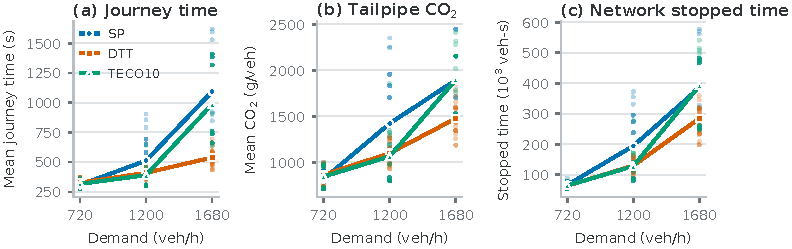
\includegraphics[width=\linewidth]{figures/fig2_performance.pdf}
\caption{Policy outcomes against demand. Lines are means over the eight contexts at
each demand level; faint points are individual runs. The three panels separate the two
primary criteria from the system-level congestion diagnostic. The policies are
near-indistinguishable at 720\,veh/h and separate sharply above it.}
\label{fig:performance}
\end{figure}

\begin{figure}[tb]
\centering
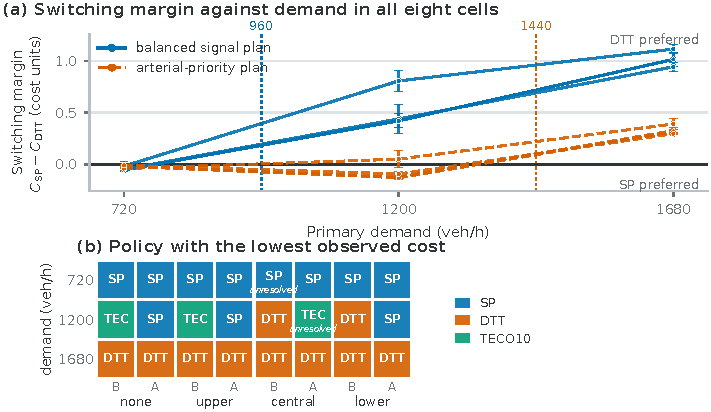
\includegraphics[width=\linewidth]{figures/fig3_regime.pdf}
\caption{(a) The switching margin of Eq.~\eqref{eq:margin} in all eight
restriction--signal cells; error bars are $\pm2$ standard errors over three paired seeds
and are descriptive, not a significance test. Dotted lines mark the two demand
thresholds fitted by the selection rules of Section~\ref{sec:selection}. (b) The policy
with the lowest observed cost in each context; the two contexts whose margin is not
resolved against replication dispersion are marked.}
\label{fig:regime}
\end{figure}

\begin{table}[htb]
\centering\footnotesize
\caption{Switching margin $m_s$ with its standard error over three paired seeds.
Negative values favour SP. The bracket is the interval of the tested demand grid in
which the sign changes; it is not a threshold estimate. $\dagger$ marks the two contexts
where $|m_s|\le 2\,\mathrm{SE}$.}
\label{tab:margin}
\setlength{\tabcolsep}{2.9pt}
\begin{tabular}{@{}llrrrrrrl@{}}
\toprule
& & \multicolumn{2}{c}{720\,veh/h} & \multicolumn{2}{c}{1200\,veh/h}
& \multicolumn{2}{c}{1680\,veh/h} & \\
\cmidrule(lr){3-4}\cmidrule(lr){5-6}\cmidrule(lr){7-8}
Signal & Restr. & $m_s$ & SE & $m_s$ & SE & $m_s$ & SE & Bracket\\
\midrule
Bal & none & $-0.0551$ & 0.0064 & $+0.4204$ & 0.0334 & $+1.0139$ & 0.0323 & (720,\,1200]\\
Bal & upper & $-0.0515$ & 0.0071 & $+0.4382$ & 0.0697 & $+0.9418$ & 0.0232 & (720,\,1200]\\
Bal & central & $-0.0195$ & 0.0220$^{\dagger}$ & $+0.8056$ & 0.0502 & $+1.1137$ & 0.0233 & (720,\,1200]\\
Bal & lower & $-0.0562$ & 0.0058 & $+0.4196$ & 0.0334 & $+1.0134$ & 0.0323 & (720,\,1200]\\
\midrule
Art & none & $-0.0184$ & 0.0046 & $-0.1269$ & 0.0101 & $+0.3249$ & 0.0162 & (1200,\,1680]\\
Art & upper & $-0.0198$ & 0.0057 & $-0.1318$ & 0.0019 & $+0.3165$ & 0.0112 & (1200,\,1680]\\
Art & central & $-0.0423$ & 0.0015 & $+0.0488$ & 0.0423$^{\dagger}$ & $+0.3893$ & 0.0250 & (720,\,1200]\\
Art & lower & $-0.0110$ & 0.0054 & $-0.0954$ & 0.0129 & $+0.2952$ & 0.0052 & (1200,\,1680]\\
\bottomrule
\end{tabular}
\end{table}

The structure is systematic rather than confined to one configuration: at 720\,veh/h the
margin is negative in all eight cells and at 1680\,veh/h positive in all eight. Over the
full portfolio, SP has the lowest observed cost in all eight low-demand contexts and DTT
in all eight high-demand contexts, while the intermediate level splits three ways --- SP
in three contexts, TECO10 in three and DTT in two. All three portfolio members win
somewhere, which establishes complementarity in the sense of Section~3.3; what that is
worth is a separate question (Section~\ref{sec:value}).

The signal plan displaces the crossing. Under balanced timing the margin has already
changed sign by 1200\,veh/h in all four restriction configurations; under
arterial-priority timing it is still negative at 1200\,veh/h in three of four and changes
sign only by 1680\,veh/h. The mean margin at 1200\,veh/h is $+0.5209$ under balanced
timing against $-0.0763$ under arterial priority, a difference of $0.5972$ cost units, so
the displacement is at least one full step of the grid, 480\,veh/h; the grid cannot say
how much more. The approach is also not uniform: under balanced timing the margin
increases with demand in all four cells, whereas under arterial priority it
\emph{decreases} from 720 to 1200\,veh/h in three of four cells before rising sharply.
Restriction location moves the margin very little --- the four balanced cells at
1200\,veh/h span $+0.4196$ to $+0.8056$, three of them within $0.02$ of each other ---
which foreshadows the feature ablation of Section~\ref{sec:selection}.

\subsection{Resolution of the Switching Boundary}
\label{sec:noise}

The experiment brackets the sign change but does not locate it
(Section~\ref{sec:boundary-exp}). What the completed data establish is that the brackets
rest on margins large relative to replication dispersion: 22 of the 24 margins in
Table~\ref{tab:margin} satisfy $|m_s|>2\,\mathrm{SE}(m_s)$, the smallest ratio among
those being 2.03. The two exceptions are the balanced central-restriction context at
720\,veh/h ($m=-0.0195$, $\mathrm{SE}=0.0220$) and the arterial central-restriction
context at 1200\,veh/h ($m=+0.0488$, $\mathrm{SE}=0.0423$). These are exactly the two
contexts in which the sign of the margin differs across the three seeds, so the
descriptive criterion and the direct seed-by-seed check agree. This also explains the one
cell that breaks the signal-plan pattern: the arterial central cell is assigned the
$(720,1200]$ bracket on the strength of a margin whose sign three replications do not
agree on, so seven of the eight cells have a resolved bracket and the eighth does not.

Dispersion is not uniform: the standard error of the margin has a median of 0.0057 cost
units at 720\,veh/h, 0.0334 at 1200\,veh/h and 0.0232 at 1680\,veh/h, with its maximum,
0.0697, also at 1200\,veh/h. Replication noise is largest precisely in the band where the
ordering changes --- the band in which a decision is hardest and, as the next subsection
shows, the one carrying most of the available decision value.

\subsection{Decision Value of Adaptation}
\label{sec:value}

Complementarity is established, but its value is modest. Over the 24 contexts the single
best fixed policy is DTT, with mean decision regret 0.03018 cost units; fixed SP and
fixed TECO10 cost 0.31825 and 0.20757. Under leave-one-context-out the depth-3 selector
attains mean regret 0.00606, chooses the lowest-cost policy in 21 of 24 contexts and is
within 1\,\% of the context optimum in 22 of 24, so by Eq.~\eqref{eq:headroom} it captures
$G=(0.03018-0.00606)/0.03018=0.799$: 79.9\,\% of the available decision headroom.

This percentage is a decision statistic and nothing else. It is \emph{not} a 79.9\,\%
reduction in travel time, emissions or any physical quantity. In physical terms the
selected policies average 412.17\,s and 1114.64\,g per vehicle against 425.17\,s and
1145.36\,g under fixed DTT --- 13.00\,s (3.06\,\%) and 30.71\,g (2.68\,\%) lower over the
evaluated contexts, with a hindsight bound of 409.25\,s and 1106.12\,g. The decision
statistic says how much of the attainable improvement was realised; the physical figures
say how large the attainable improvement was.

The headroom is highly localised (Fig.~\ref{fig:decision}b). At 1680\,veh/h DTT is best
in all eight contexts, so there is nothing for adaptation to win: the fixed policy has
exactly zero mean regret and the entire penalty in that regime belongs to choosing the
\emph{wrong} fixed policy, which costs 0.67611 under SP. At 720\,veh/h the fixed policy
carries 0.03422 and the selector removes all of it; the transition band carries 0.05633,
of which the selector removes about two thirds, leaving 0.01818. Weighted by the eight
contexts in each regime, 37.8\,\% of the total headroom sits at low demand, 62.2\,\% in
the transition band and none at high demand.

Two conclusions follow and they point in different directions. Adaptation is worth having,
but it is worth much less than choosing the right fixed policy: the difference in mean
regret between the best and worst fixed policy, 0.28807 cost units, is nearly ten times
the entire headroom adaptation competes for. The first-order operational result is about
the fixed choice; adaptation is a second-order refinement concentrated in one demand
band.

\subsection{Noise and Effect Size}

A headroom of 0.03018 should be checked against the dispersion of the benchmark that
produced it. Recomputing the whole decision analysis independently within each seed block
gives 0.04138, 0.03035 and 0.02959 cost units, a mean of 0.03377 with a standard error of
0.00381 across blocks. The quantity the selector competes for is therefore roughly eight
times the dispersion of its own estimate --- enough for the comparison above to be
meaningful, but not enough to treat its fifth decimal place as stable; the differences
that matter are the order-of-magnitude ones, 0.318 against 0.030 against 0.006. At context
level the picture is less reassuring in the transition band, where the median absolute
margin is 0.2757 cost units against a median standard error of 0.0334 but individual
ratios run down to the two unresolved contexts above, and all three of the selector's
remaining errors fall in that band. The difficulty is concentrated where the data are
noisiest --- expected for a boundary-detection task, and the main reason the residual
20\,\% of the headroom is not recovered.

\subsection{Mechanistic Interpretation}

The reversal has a consistent physical description (Table~\ref{tab:mechanism}). SP's route
is about 8\,\% shorter than DTT's and that advantage is essentially constant across
regimes; what changes is the cost of using the shorter corridor. Between the lowest and
highest demand, implied in-network mean speed falls from 37.80 to 18.31\,km/h for SP, a
loss of 51.6\,\%, against 38.43 to 23.80\,km/h for DTT, a loss of 38.1\,\%, while emission
intensity rises from 255.1 to 590.7\,g/km for SP but only from 248.5 to 423.2\,g/km for
DTT. A fixed structural advantage is overtaken by a growing congestion penalty: at
720\,veh/h the policies achieve almost identical speeds and queueing, so DTT's longer route
is not compensated, whereas as demand rises the shortest corridor degrades faster than the
alternatives and the margin flips sign. Under arterial priority that corridor receives a
larger green share, consistent with the later crossing in Table~\ref{tab:margin}.

\begin{table}[htb]
\centering\small
\caption{Mechanism decomposition: SP minus DTT, averaged over the eight contexts at each
demand level. A negative distance difference means SP's route is shorter; a positive time
difference means SP is slower.}
\label{tab:mechanism}
\begin{tabular}{@{}lrrrrrr@{}}
\toprule
Demand & $\Delta$distance & $\Delta$in-network & $\Delta$insertion & $\Delta$journey
& $\Delta$\CO & $\Delta$stopped\\
& (m) & time (s) & delay (s) & time (s) & (g/veh) & (veh-s/veh)\\
\midrule
720\,veh/h & $-250.3$ & $-17.9$ & $0.0$ & $-17.9$ & $-44.7$ & $+6.4$\\
1200\,veh/h & $-288.0$ & $+84.8$ & $+18.1$ & $+102.8$ & $+322.5$ & $+104.1$\\
1680\,veh/h & $-277.2$ & $+113.7$ & $+441.2$ & $+554.9$ & $+416.9$ & $+114.3$\\
\bottomrule
\end{tabular}
\end{table}

This is a decomposition, not a causal identification. The experiment varies demand and
green split but does not isolate movement-level mechanisms, and the per-run aggregates
contain no per-approach delay, stop count or route-share breakdown.

\subsection{Context-Aware Selection}
\label{sec:selection}

\begin{figure}[tb]
\centering
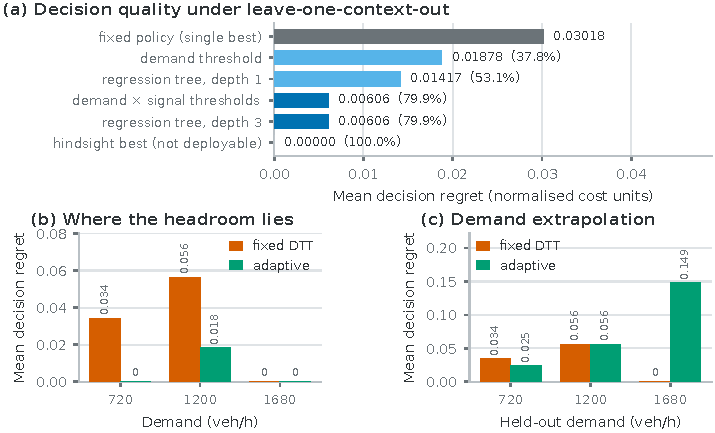
\includegraphics[width=\linewidth]{figures/fig4_decision.pdf}
\caption{(a) Mean decision regret of every rule in the ladder under
leave-one-context-out, with the percentage of headroom captured. (b) Where the headroom
lies: at 1680\,veh/h the fixed policy is already optimal. (c) Leave-one-demand-out. When
the withheld demand level lies above the fitted support the adaptive rule is
substantially worse than the fixed policy it replaces.}
\label{fig:decision}
\end{figure}

\begin{table}[htb]
\centering\small
\caption{Selection rules under leave-one-context-out. Everything --- reference scales,
thresholds, tree and the identity of the best fixed policy --- is refitted inside each
fold. Mean and max are decision regret in normalised cost units; ``lowest cost'' counts
contexts in which the chosen policy is the observed best; ``captured'' is $G(\pi)$ of
Eq.~\eqref{eq:headroom}.}
\label{tab:ladder}
\begin{tabular}{@{}llrrcr@{}}
\toprule
& Rule & Mean & Max & Lowest cost & Captured\\
\midrule
R0 & Single best fixed policy & 0.03018 & 0.13176 & 10/24 & ---\\
R1 & Demand threshold & 0.01878 & 0.13176 & 18/24 & 37.8\,\%\\
R3 & Regression tree, depth 1 & 0.01417 & 0.10079 & 17/24 & 53.1\,\%\\
R2 & Demand $\times$ signal thresholds & 0.00606 & 0.11545 & 21/24 & 79.9\,\%\\
R4 & Regression tree, depth 3 & 0.00606 & 0.11545 & 21/24 & 79.9\,\%\\
R5 & Hindsight best (not deployable) & 0.00000 & 0.00000 & 24/24 & 100\,\%\\
\bottomrule
\end{tabular}
\end{table}

Table~\ref{tab:ladder} and Fig.~\ref{fig:decision}a report the ladder under the identical
held-out protocol. The central result is the equality of rows R2 and R4: a rule with two
free parameters, one demand threshold per signal plan, reproduces the regression tree
exactly --- same mean regret, same maximum regret, the same 21 contexts chosen correctly.
The fitted models explain why: in all 24 folds the tree splits first on demand at
1440\,veh/h, then on signal plan, then on demand again at 960\,veh/h, while the explicit
rule fits thresholds of 960\,veh/h under balanced timing and 1440\,veh/h under arterial
priority in every fold. The two rules are the same rule.

This bounds what the learned model contributes: the 79.9\,\% is produced by the regime
structure of Section~6.2, not by model capacity, and a practitioner would obtain the same
decisions from two numbers written on a page. Feature ablation agrees --- removing the
restriction configuration leaves the result unchanged at 79.9\,\%, whereas removing the
signal plan reduces it to 72.9\,\%. The ladder also separates prediction quality from
decision quality: the depth-3 model predicts poorly in absolute terms, with held-out mean
absolute error of 44.6\,s in journey time and 82.4\,g in \CO\ against benchmark means of
542.8\,s and 1263.5\,g, yet chooses the lowest-cost policy in 21 of 24 contexts, because
errors that preserve the ordering of three policies cost nothing. This is the
predict-then-optimise distinction of~\cite{elmachtoub2022smart} in a traffic setting, and
it means reporting the selector's regression accuracy would misdescribe its usefulness.

\paragraph{The extrapolation boundary.}
The leave-one-demand-out experiment reverses the conclusion (Fig.~\ref{fig:decision}c).
Pooled over the three folds, mean regret rises to 0.07649, above the 0.03018 of the fixed
policy: applied this way the procedure is worse than doing nothing adaptive. The folds are
not equivalent. With 1200\,veh/h withheld the test point lies between two training levels
and the selector reproduces the fixed-policy regret of 0.05633 exactly, gaining nothing;
with 720\,veh/h withheld it never sees a context in which SP is optimal and incurs 0.02456
against 0.03422, slightly better only because the fixed policy is also wrong there; and
with 1680\,veh/h withheld the test point lies above the training range, DTT is optimal in
all eight withheld contexts, the selector assigns TECO10 to half of them, and it incurs
0.14856 where the fixed policy incurs zero.

The failure is specific and diagnosable rather than general: a tree cannot extrapolate,
returning beyond the largest training value of a feature the prediction of its outermost
leaf, which here was fitted where TECO10 was competitive. Interpolation inside a
represented range is safe in this benchmark, extrapolation beyond it is not, and a model
that produces a prediction outside its support is not thereby producing a usable one.

\subsection{Multi-Criteria and Pareto Structure}
\label{sec:multicriteria}

\begin{figure}[tb]
\centering
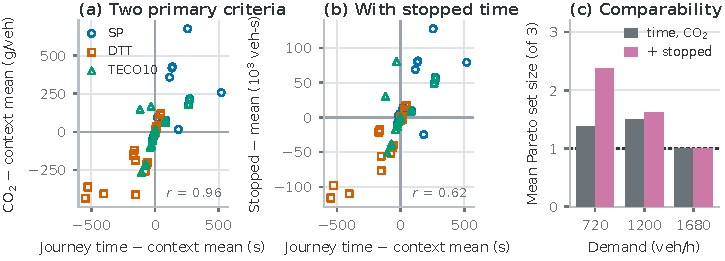
\includegraphics[width=\linewidth]{figures/fig5_pareto.pdf}
\caption{Multi-criteria structure. (a, b) Policy outcomes expressed as deviations from
their own context mean, which isolates the comparison that decides a context; $r$ is the
mean within-context correlation across the three policies. (c) Mean number of
non-dominated policies per context, with and without the congestion axis.}
\label{fig:pareto}
\end{figure}

Whether a preference model does any work depends on how independent the criteria are.
Within a context --- the comparison that determines which policy wins --- the mean
correlation between mean journey time and \CO\ across the three policies is 0.96
(Fig.~\ref{fig:pareto}a), so the two primary criteria are close to collinear, which is why
the weight sweep below changes nothing; the corresponding correlation between journey time
and network stopped vehicle-time is 0.62 (Fig.~\ref{fig:pareto}b), so the congestion
diagnostic carries information the primary criteria do not.

Treating that diagnostic as a third axis changes comparability but not the decision. Under
the two primary criteria the mean Pareto set contains 1.29 of the three policies and 17 of
24 contexts have a single non-dominated policy; adding stopped vehicle-time raises the
mean set to 1.67 and leaves only 12 such contexts, the effect concentrated at low demand
where the mean set size rises from 1.38 to 2.38. At 1680\,veh/h it remains 1.00 under
both, DTT dominating outright on all three axes. Crucially, the policy chosen by the
primary rule is non-dominated in the three-criterion sense in all 24 contexts, so the
reported decisions are never Pareto-dominated once congestion is included. An equal-weight
additive rule over all three criteria agrees with the primary rule in 22 of 24 contexts
--- the exceptions being the balanced central-restriction context at 720\,veh/h and the
balanced upper-restriction context at 1200\,veh/h --- and ranking by stopped vehicle-time
alone agrees in 18 of 24. The congestion diagnostic therefore reduces the \emph{confidence}
with which policies can be ordered at low demand, where they differ little on any axis,
without altering the regime structure or the decisions. That is also why it was not
promoted to a primary criterion: it would have changed the meaning of the reported
decisions while changing almost none of them.

\subsection{Robustness and Negative Controls}
\label{sec:robust}

\begin{table}[htb]
\centering\small
\caption{Sensitivity checks under the primary protocol. ``Captured'' is the fraction of
headroom recovered; ``labels changed'' counts contexts in which the preferred policy
differs from the primary analysis. All 15 depth/leaf settings capture positive headroom.
The two negative controls are described in the text. $^{\ast}$On the in-network scale the
headroom is 0.03305 rather than 0.03018.}
\label{tab:robust}
\setlength{\tabcolsep}{4pt}
\begin{tabular}{@{}lll@{}}
\toprule
Variation & Captured & Labels changed\\
\midrule
Primary analysis (depth 3, leaf 2, $w=0.5$) & 79.9\,\% & ---\\
Depth $\in\{1,2,3,4,\infty\}\times$ leaf $\in\{1,2,3\}$ & 50.9--79.9\,\% & --- \\
Weight $w_{\text{time}}$ swept $0\rightarrow1$ & 78.1--81.7\,\% & 0 of 24 decisions\\
Seed-block hold-out, three blocks & 60.8, 67.7, 90.2\,\% & ---\\
Training-only scoring scales & 79.8\,\% & ---\\
In-network time replaces journey time & 80.1\,\%$^{\ast}$ & 0 of 24\\
95th percentile replaces the mean & --- & 2 of 24\\
Route distance as a third criterion & --- & 0 of 24\\
Stopped vehicle-time as a third criterion & --- & 2 of 24\\
\bottomrule
\end{tabular}
\end{table}

Table~\ref{tab:robust} collects the checks of Section~5.4; the held-out advantage survives
all of them. Both negative controls fire, and both constrain the paper's own claims.

The emission-forecast control is the reason ECO is not in the decision portfolio. Its
aggregate accuracy is acceptable --- selected-path emission WAPE of 14.71\,\% against a
25\,\% criterion and signed bias $-0.32$\,\% against a 10\,\% criterion --- yet in a
fixed-replay probe over all 29 admissible routes it identified the best route in only 3 of
8 panels, with a mean relative selection loss of 21.62\,\% and a worst case of 78.16\,\%.
Good average forecast accuracy did not produce good route choices, the
accuracy--decision gap of Section~\ref{sec:selection} in the opposite direction. ECO is
also outcome-identical to SP in 21 of 24 contexts here. Neither observation is evidence
that eco-routing is ineffective in general; both are statements about this estimator in
this environment.

The preference-model control is a negative result about this study's own apparatus:
sweeping the time weight from 0 to 1 leaves every selector decision unchanged and changes
the hindsight winner in a single context, so the multi-criteria layer is doing almost no
work here. Adding further multi-criteria methods would produce agreement among methods
rather than evidence about the traffic system, and we therefore report the additive model
as a transparent definition of ``preferred'' rather than as a contribution.

\subsection{Implications and Limitations}

The three questions of Section~1 receive different answers, and the differences are the
point: the preferred policy changes with regime, the decision value of that change is real
but small and localised, and the recovery is deployable only inside the represented
regimes. For practice this suggests a modest design --- commit first to the right fixed
policy, which is where most of the available cost sits, then add adaptation as two demand
thresholds conditioned on the active signal plan, with a declared operating domain
monitored against the demand range used to fit it and a fixed-policy fallback outside it.

The limitations are concrete. \emph{External validity:} one synthetic topology, one primary
origin--destination structure, specified rather than calibrated lane capacities and a
homogeneous fleet, so the brackets, headroom and capture percentages are benchmark-specific
quantities. \emph{Resolution:} 24 contexts, three replications and a demand grid of
480\,veh/h; the experiment brackets the preference change rather than locating it, the runs
that would locate it were not available (Section~\ref{sec:boundary-exp}), two of the 24
margins are unresolved, and leave-one-context-out estimates procedure quality on folds that
share most of their training contexts. \emph{Behaviour:} restrictions are announced,
compliance is complete and routes are assigned once at departure, so nothing here speaks to
heterogeneous compliance, en-route control, or the feedback that would arise if a large
share of traffic followed the same guidance. \emph{Criteria and measurement:} the two
primary criteria are nearly collinear here, so the preference model is close to inert;
journey time includes insertion delay while in-network \CO\ does not, which leaves the
ordering unaffected but not the absolute values at the highest demand; and the congestion
diagnostic is measured over all vehicles rather than the cohort. \emph{Mechanism:} the
per-run aggregates support a consistent decomposition of the reversal but not a causal
attribution to particular movements or signal phases. \emph{Scope:} the review is targeted
rather than systematic, and the paper accordingly claims no priority.

\section{Conclusion}

This study treats the choice of a routing policy as a context-dependent decision problem
and evaluates it on a controlled signalised benchmark of 432 completed SUMO runs over 24
contexts. Shortest-distance routing has the lowest observed cost in all eight low-demand
contexts and dynamic travel-time routing in all eight high-demand contexts, with the
crossing displaced by at least one demand step under arterial-priority timing, and all
three portfolio policies win somewhere, so the portfolio is complementary.

Complementarity, however, is not decision value. The single best fixed policy leaves only
0.03018 normalised cost units of headroom, of which a leave-one-context-out selector
recovers 79.9\,\% --- a share of attainable decision quality, not a physical improvement
rate; the corresponding physical differences are 13.00\,s and 30.71\,g per vehicle, while
choosing the worst rather than the best fixed policy costs 0.28807 units. A two-threshold
rule on demand and signal plan matches the fitted regression tree exactly, so the
recoverable value comes from the regime structure and not from model capacity.

Decision value is in turn not deployability. When an entire demand regime is withheld,
pooled regret rises to 0.07649, above the fixed-policy benchmark, and in the fold that
extrapolates above the training range the adaptive rule incurs 0.14856 where the fixed
policy incurs nothing. The recommendation is therefore conditional and operationally
specific: context-dependent routing-policy selection is worth deploying only within an
explicitly declared regime domain, implemented as a small number of interpretable
thresholds, with a fixed-policy fallback whenever the operating context leaves it.
Establishing where inside the observed brackets the preference actually changes requires
intermediate-demand simulations on this same network, which remain to be run.

\bibliographystyle{splncs04}
\bibliography{references}

\end{document}
